\section{Evaluation}
The following evaluated training processes have been carried out on two GPUs as described in section \ref{sec:hardware}.
In order to make optimal use of the available GPUs, the training and evaluation process have been performed independently.
More specifically, all trained models are saved after each finished epoch in order to load it on a separate machine and evaluate it.
That way training can seamlessly continue while the last saved model is loaded and evaluated in parallel on the regarding training set.


\subsection{Input Pipeline with multiple GPUs}
To evaluate the training speed up by using multiple GPUs with an asynchronous input pipeline, we measure the number of training input clips that can be processed per second in different setups.
Specifically, processing an input during training includes calculating the forward pass through the network, calculating the weight updates and applying them to the model.
In the case of multiple GPUs, the calculated weight updates of the individual GPUs need to be averaged to obtain a global model update after each training step as described in section \ref{sec:multi_gpu}.
For the incorporated \textit{C3D} model an input clip denotes a $16 \times 112 \times 112 \times 3$ video volume, i.e. $16$ frames of resolution $112 \times 112$ pixel in $3$ channels (RGB).

During training without input pipeline (denoted as \textit{no IP} in table \ref{tab:training_speed}), input processing and training are executed sequentially: an input is first pre-processed and then fed into the model for training in the same thread.
This yields the disadvantage, that the GPUs need to wait for the input clips to be ready for further processing.
This time however depends on the dataset, since e.g. video decoding time depends on the video quality.
Training with input pipeline (denoted as \textit{IP} in table \ref{tab:training_speed}) incorporates a FIFO Queue which is fed from four threads asynchronously as described in \ref{subsec:inputpipeline}.
That way an input clip is ready whenever needed, if the pre-processing threads are faster than the GPUs.

All measurements are taken from training on UCF-101, which has shown to be the fastest dataset to be decoded in comparison to Kinetics and Charades.
Speed measurements on the CPU were only obtained for a batchsize of 10 without input pipeline, since the result already indicates the infeasibility of training on the CPU and bigger batchsizes were not processible due to memory limitations.

\begin{table}[H]
    \centering
    \renewcommand{\arraystretch}{1.5}
    %\scriptsize
    \caption*{\textbf{Training Speed in clips/second}}
    \vspace{8pt}
    \begin{tabulary}{\textwidth}{R|C C|C C|C C}
    %\multirow{2}{*}{clips / s}
    & \multicolumn{2}{c|}{\textbf{batch = 10 clips}} & \multicolumn{2}{c|}{\textbf{batch = 20 clips}} & \multicolumn{2}{c}{\textbf{batch = 40 clips}} \\
    & no IP & IP & no IP & IP & no IP & IP \\
    \hline\hline
    CPU & 0.08 \newline$\pm$ 0.01 & \hfill & & & & \\
    GPU & 14.04 \newline$\pm$ 0.93 & 13.59 \newline$\pm$ 1.54 & 14.94 \newline$\pm$ 0.66 & 14.74 \newline$\pm$ 0.92\\
    2 $\times$ GPU & 8.39 \newline$\pm$ 1.29 & 16.70 \newline$\pm$ 0.71 & 13.66 \newline$\pm$ 0.61 & 22.36 \newline$\pm$ 0.58 & 15.07 \newline$\pm$ 0.73 & 26.32 \newline$\pm$ 0.67 \\
    \end{tabulary}
    \caption{Training speed for different batchsizes with and without multi-threaded queue-based input pipeline (IP and no IP) measured for 100 training steps each.}
    \label{tab:training_speed}
\end{table}

The results in table \ref{tab:training_speed} indicate:
\begin{enumerate}
\item Training on the CPU only is infeasible.
\item For smaller batch-sizes, i.e. $10$ or $20$ clips per batch, the overhead from averaging the gradients of multiple GPUs and communication the updates hurts training speed to a point where a single GPU is more effective.
\item A sophisticated input pipeline is not necessary for batchsizes of $10$ and $20$ clips.
We note that this is in part due to the low resolution of UCF-101 videos which results in fast decoding and therefore short pre-processing times.
\item Batchsizes of $40$ clips are only processable with two GPUs due to the doubled amount of GPU memory.
\item Two GPUs significantly benefit from an asynchronous input pipeline and perform best in this setup.
\end{enumerate}


\subsection{UCF-101 Classification without Pre-Training}
To provide a baseline for comparing the effects of pre-training with \textit{temporal order verification}, a \textit{C3D} model is trained on UCF-101 (split 1) from randomly initialized weights.
More precisely, weights are initialized from a normal distribution with mean $0$ and standard deviation of $0.01$.
\footnote{Whenever weights are initialized randomly in the following evaluations, exactly this distribution is meant and used.}
The model is trained for $23.9$k iterations, which corresponds to $100$ finished epochs at a batch-size of $40$ clips per iteration and $9,537$ videos in the training set of UCF-101.
The overall training process takes 12 hours 20 minutes and 12 seconds.
A learning rate of $10^{-5}$ was found to be the biggest possible learning rate without resulting in diverging loss.

Figure \ref{fig:ucf101scratchloss} shows the \textbf{loss} per batch for each training-step of both GPUs.
The training process clearly converges, indicated by a degrading loss towards 0 and a slope of approximately $0$ during the last iterations.

\begin{figure}[H]
    \begin{subfigure}[c]{\textwidth}
    \centering
    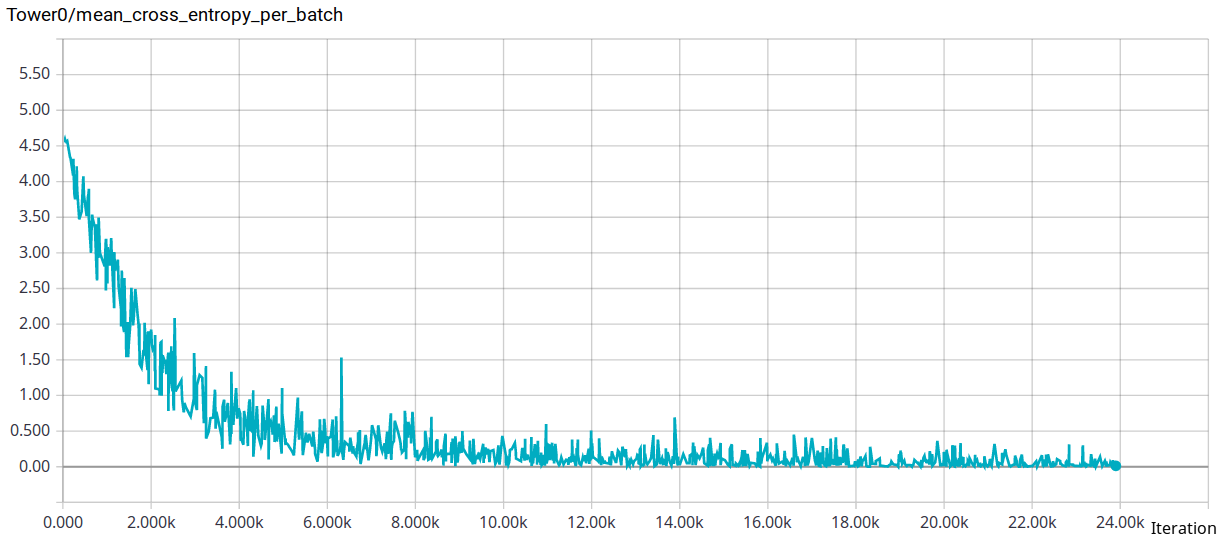
\includegraphics[width=\textwidth]{img_evaluation/ucf101_scratch/tower0crossentropy}
    \subcaption{Training loss of GPU0 (Tower0)}
    \end{subfigure}
    \begin{subfigure}[c]{\textwidth}
    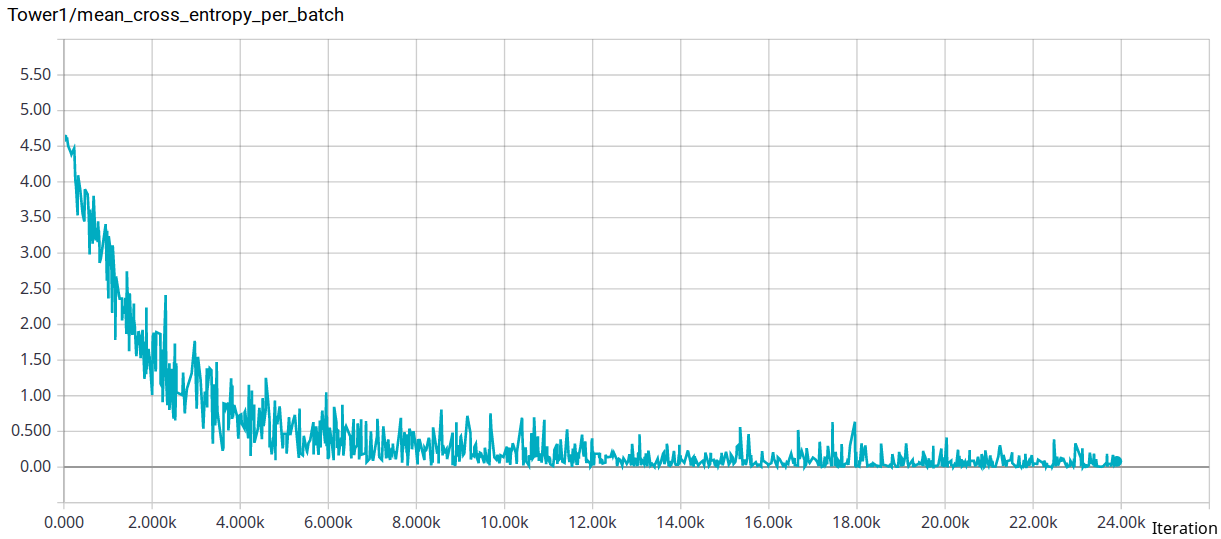
\includegraphics[width=\textwidth]{img_evaluation/ucf101_scratch/tower1crossentropy}
    \subcaption{Training loss of GPU1 (Tower1)}
    \end{subfigure}
    \caption{Training loss of the \textit{C3D} model per batch while training from randomly initialized weights on split 1 of UCF-101.}
    \label{fig:ucf101scratchloss}
\end{figure}

Figure \ref{fig:ucf101scratchaccuracy} shows the \textbf{accuracy} per batch for each training-step of both GPUs while training on UCF-101.
The training accuracy rises to near optimum during convergence of the training process.
This indicates overfitting, as we are training a deep model on a comparably small dataset (see section \ref{sec:datasets}).

To evaluate the performance of our model on the testset of UCF-101 we incorporate the evaluation strategy proposed in \cite{carreira_quo_2017}.
Test accuracy is measured by cropping consecutive center clips from the test video, feeding them to the model and averaging the individual outputs.
This way the complete temporal evolution of the video can be taken into account for calculating the test accuracy, since a variable number of clips can be averaged to cover different video lengths.
The cropped center clips can possibly overlap, i.e. an offset between the beginnings of consecutive clips can be varied.
An offset of $\omega = 16$ corresponds to no overlap, an offset of $\omega < 16$ results in $16 - \omega$ overlapping frames and an offset of $\omega > 16$ results in gaps between consecutive clips.
For our evaluation we incorporate no overlap, i.e. $\omega = 16$, as a compromise between evaluation speed and video coverage.

\textbf{Result:}\\
Epoch 65 results in the best performing model on the test-set of UCF-101 with an accuracy of $44.57\%$.
The early maximum of the test accuracy and difference between training and test accuracy confirms the conjecture, that the model is overfitting to the data.
Nevertheless, our result is comparable to the reported performance of \cite{carreira_quo_2017} ($51.6\%$ accuracy) and \cite{varol_long-term_2016} ($51.9\%$ accuracy).
Our resulting accuracy is slightly lower, since no hyperparameter-tuning has been performed as we are for now only interested in a functioning baseline to evaluate the difference against pre-training the same model with the same hyperparameters using \textit{temporal order verification}\cite{misra_shuffle_2016}.

\begin{figure}[H]
    \begin{subfigure}[c]{\textwidth}
    \centering
    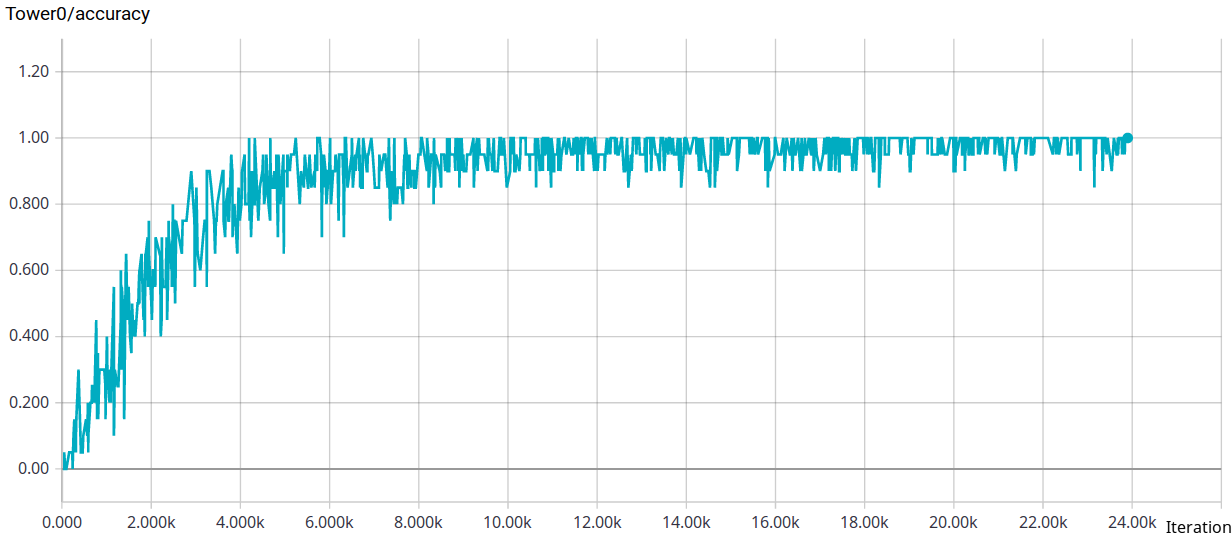
\includegraphics[width=\textwidth]{img_evaluation/ucf101_scratch/tower0accuracy}
    \subcaption{Training accuracy of GPU0 (Tower0)}
    \end{subfigure}
    \begin{subfigure}[c]{\textwidth}
    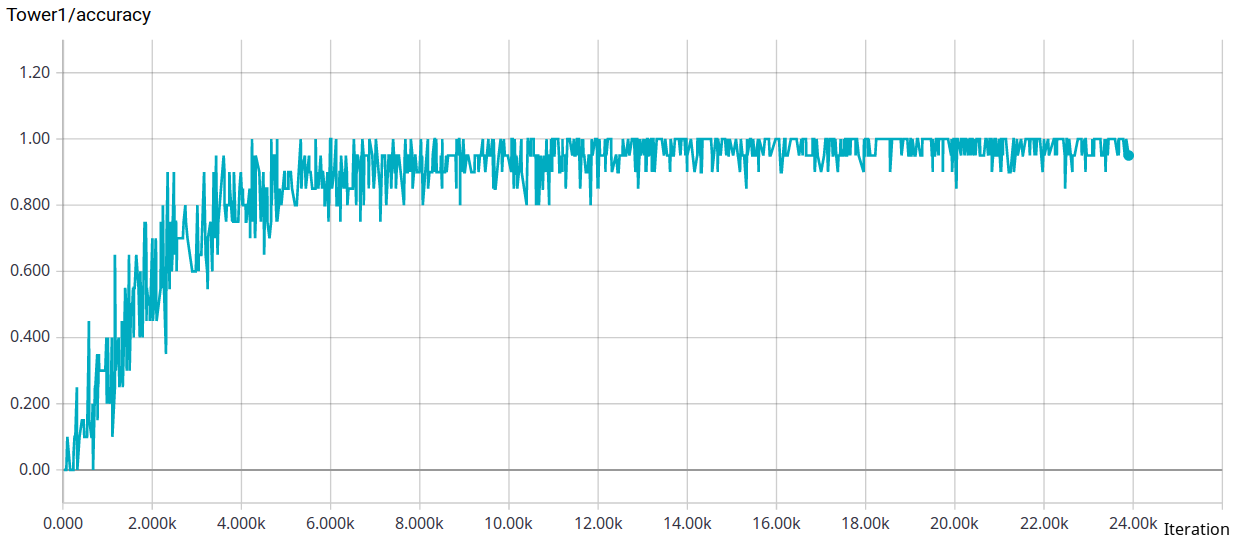
\includegraphics[width=\textwidth]{img_evaluation/ucf101_scratch/tower1accuracy}
    \subcaption{Training accuracy of GPU1 (Tower1)}
    \end{subfigure}
    \caption{Training accuracy of the \textit{C3D} model per batch while training from randomly initialized weights on split 1 of UCF-101.}
    \label{fig:ucf101scratchaccuracy}
\end{figure}


\subsection{Charades Classification without Pre-Training}
Similar to obtaining a baseline for the UCF-101 dataset, a \textit{C3D} model is trained on the Charades dataset from randomly initialized weights.
The weights are again sampled from a normal distribution with mean $0$ and standard deviation of $0.01$.
The model is trained for roughly $206.8$k iterations, which corresponds to $166$ epochs at a batch-size of $40$ clips per iterations and $49,809$ temporally localized actions in the training-set of Charades.
The training process takes 7 days 11 hours 11 minutes and 14 seconds.
A learning rate of $10^{-5}$ was found to be the biggest possible learning rate without resulting in diverging loss.

Figure \ref{fig:charadesscratchloss} shows the loss per batch for each training-step of both GPUs.
The training process did not fully converge as there is still a noticeable slope present in the last $40$k iterations.
As computation time is limited and this model is trained as a baseline, the training was stopped at this point after roughly eight days.

\begin{figure}[H]
    \begin{subfigure}[c]{\textwidth}
    \centering
    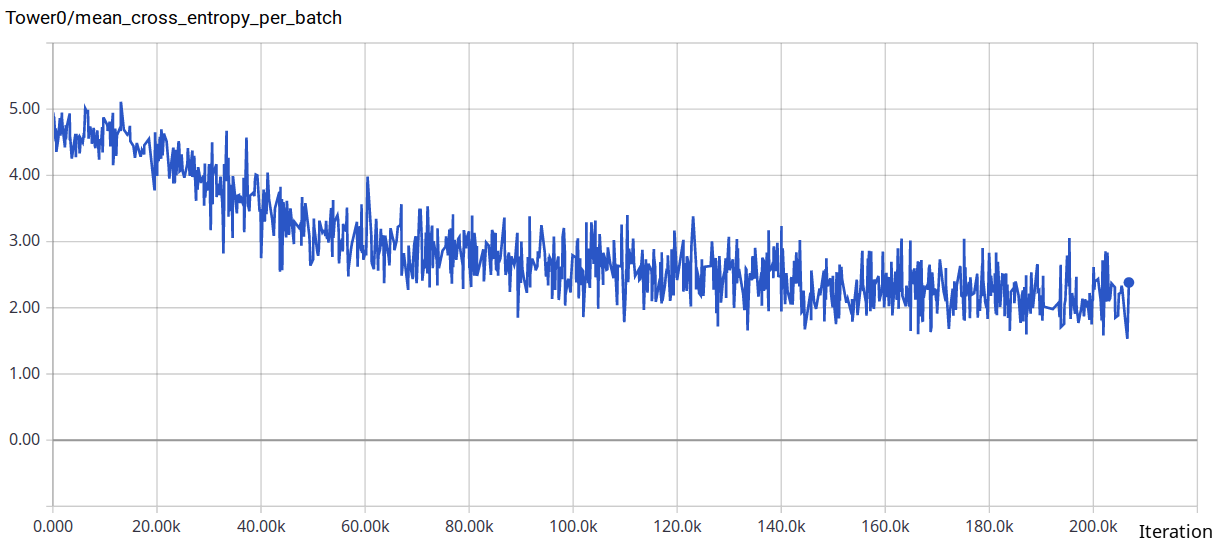
\includegraphics[width=\textwidth]{img_evaluation/charades_scratch/tower0crossentropy}
    \subcaption{Training loss of GPU0 (Tower0)}
    \end{subfigure}
    \begin{subfigure}[c]{\textwidth}
    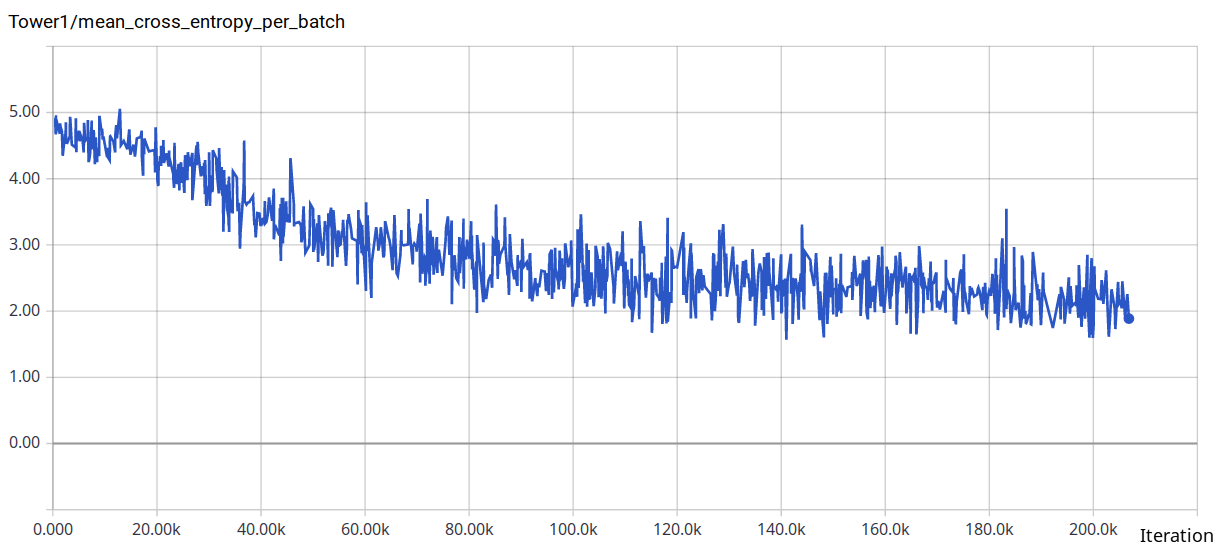
\includegraphics[width=\textwidth]{img_evaluation/charades_scratch/tower1crossentropy}
    \subcaption{Training loss of GPU1 (Tower1)}
    \end{subfigure}
    \caption{Training loss of the \textit{C3D} model per batch while training from randomly initialized weights on the Charades dataset.}
    \label{fig:charadesscratchloss}
\end{figure}

Figure \ref{fig:charadesscratchaccuracy} shows the accuracy per batch for each training-step of both GPUs on the Charades dataset.
The training accuracy starts to rise significantly after around $35$k iterations, which corresponds to $24h$ of training.
The evolution of the accuracy curve indicates, that this is a more difficult learning task than UCF-101 classification.
This is partly due to the fact, that labels are ambiguous on the Charades dataset since they can overlap for a single video as described in section \ref{subsec:charadeslabelling}.

\begin{figure}[H]
    \begin{subfigure}[c]{\textwidth}
    \centering
    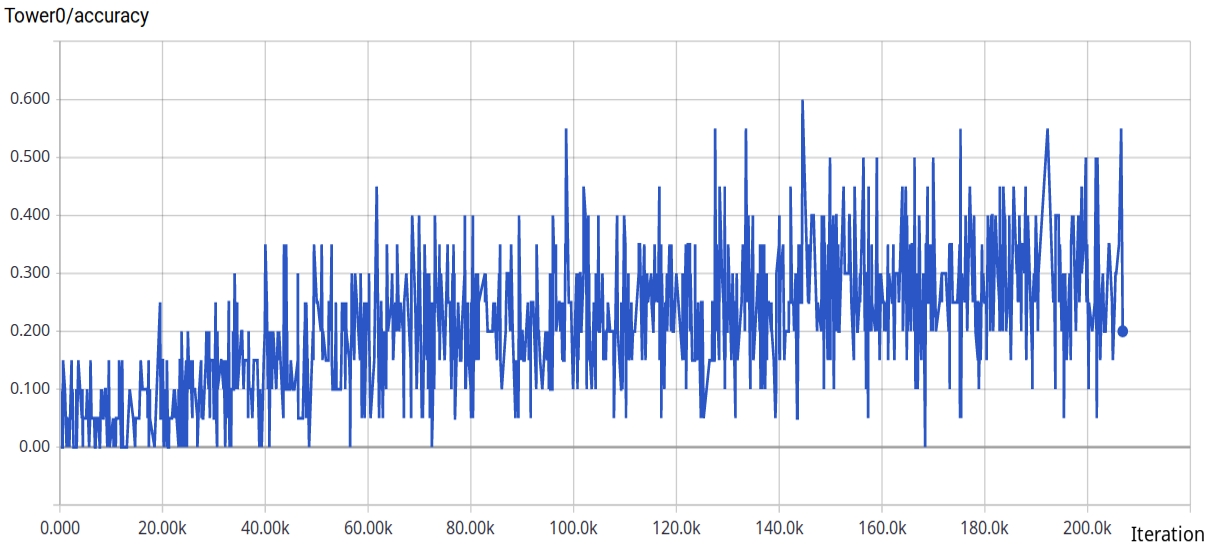
\includegraphics[width=\textwidth]{img_evaluation/charades_scratch/tower0accuracy}
    \subcaption{Training accuracy of GPU0 (Tower0)}
    \end{subfigure}
    \begin{subfigure}[c]{\textwidth}
    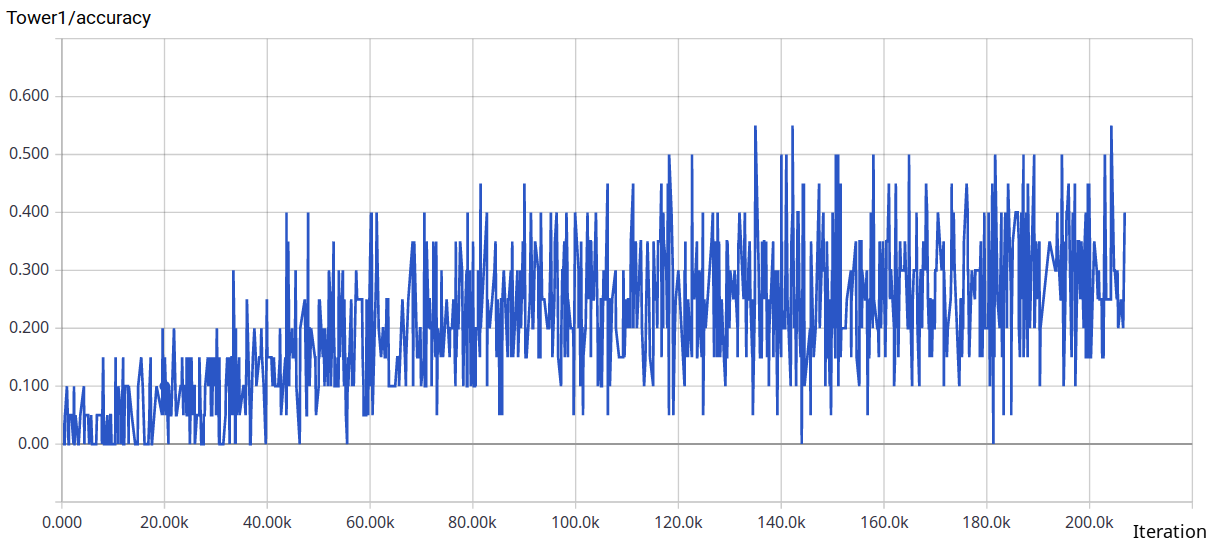
\includegraphics[width=\textwidth]{img_evaluation/charades_scratch/tower1accuracy}
    \subcaption{Training accuracy of GPU1 (Tower1)}
    \end{subfigure}
    \caption{Training accuracy of the \textit{C3D} model per batch while training from randomly initialized weights on the Charades dataset.}
    \label{fig:charadesscratchaccuracy}
\end{figure}

Since labels are ambiguous, test accuracy is not an appropriate performance measure any more.
Therefore \textit{mean average precision}\cite{zhu_recall_2004} was established as standard performance measure on the charades dataset.
To evaluate the performance of our model on the test-set of Charades we again incorporate the evaluation strategy proposed in \cite{carreira_quo_2017}.
Network outputs per test video are obtained by cropping consecutive center clips from the test video, feeding them to the model and averaging the individual outputs.
The mean average precision (mAP) for classifying Charades videos is calculated from the network outputs for all test videos using the provided evaluation script (see section \ref{subsec:charadeslabelling}).

\textbf{Result:}
The \textit{C3D} network trained from randomly initialized weights yields a mAP of $9.01\%$ after epoch 146.
This result is comparable to the reported mAP ($10.9\%$) in the original Charades publication by \textcite{sigurdsson_hollywood_2016}, as described in section \ref{subsubsec:charades_baselines}.
\textcite{sigurdsson_hollywood_2016} use a \textit{C3D} model pre-trained on Sports-1M\cite{karpathy_large-scale_2014} while ours is trained from random weights, which explains the difference in performance.

\subsection{Pre-Training on Kinetics}
This section evaluates \textit{temporal order verification} with the previously introduced methods of sampling positive (\textit{correct temporal order}) and negative (\textit{incorrect temporal order}) input clips from the Kinetics dataset.
A \textit{C3D} model is pre-trained on these three methods, which are further called \textit{method 1, 2 and 3}.
\bigskip

\textbf{Method 1}\\
Pre-training of a \textit{C3D} model is performed with sampled input clips, that are split in three equal parts which are then randomly permuted to generate a negative input sample or kept in place to generate a positive input sample.

Figure \ref{fig:pretrain1} illustrates the pre-training process by showing the training accuracy and training loss for each input batch per training step on GPU0.
In the following evaluation results for GPU1 are omitted to not unnecessarily lengthen this report.

\begin{figure}[H]
    \begin{subfigure}[c]{\textwidth}
    \centering
    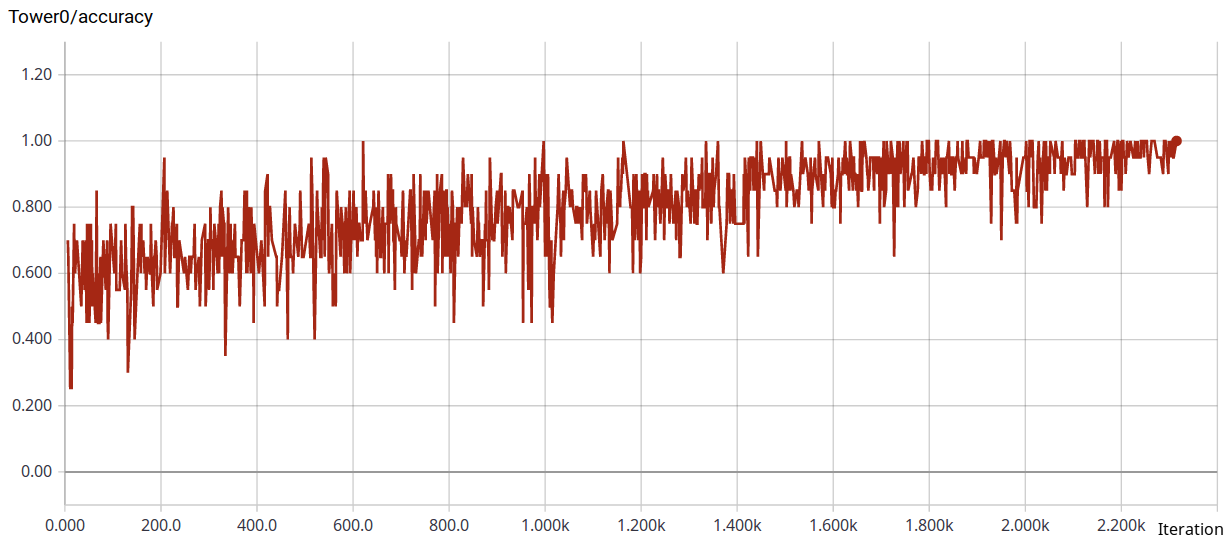
\includegraphics[width=\textwidth]{img_evaluation/pretrain1/tower0accuracy}
    \subcaption{Training accuracy of GPU0 (Tower0)}
    \end{subfigure}
    \begin{subfigure}[c]{\textwidth}
    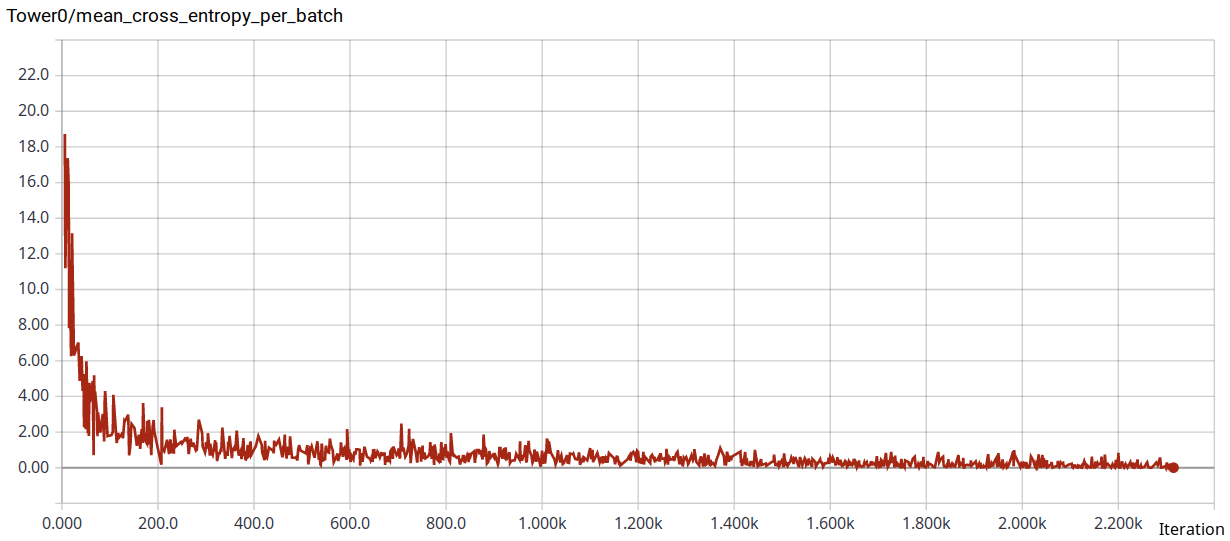
\includegraphics[width=\textwidth]{img_evaluation/pretrain1/tower0crossentropy}
    \subcaption{Training loss of GPU0 (Tower0)}
    \end{subfigure}
    \caption{Pre-training process by \textit{temporal order verification} using input sampling method 1.}
    \label{fig:pretrain1}
\end{figure}

As figure \ref{fig:pretrain1} illustrates, the training process converges after only $2.2$k iterations, which is extremely fast considering previous training times.
This goes against the observation in the original \textit{temporal order verification} publication\cite{misra_shuffle_2016}, which reports pre-training for $100$k iterations.
Since here a more complex 3D CNN is trained, we assume even longer pre-training times.
This indicates that the model learned to just focus on the regions where cuts can occur, as diving dividing the input clip in only three equal parts generate cuts at distinct locations.
Due to limited computation time and this obvious flaw in \textit{method 1}, we therefore abandon this method and focus on \textit{method 2} and \textit{3}.
\bigskip

\textbf{Method 2}\\
This input sampling improves over the previous sampling \textit{method 1} in that a cut from permuting the input clip can potentially occur between any two frames.
Figure \ref{fig:pretrain2} illustrates the pre-training process by showing the training accuracy and loss for each batch per training step on GPU0.
Results on GPU1 are again similar enough to be omitted in this report.

\begin{figure}[H]
    \begin{subfigure}[c]{\textwidth}
    \centering
    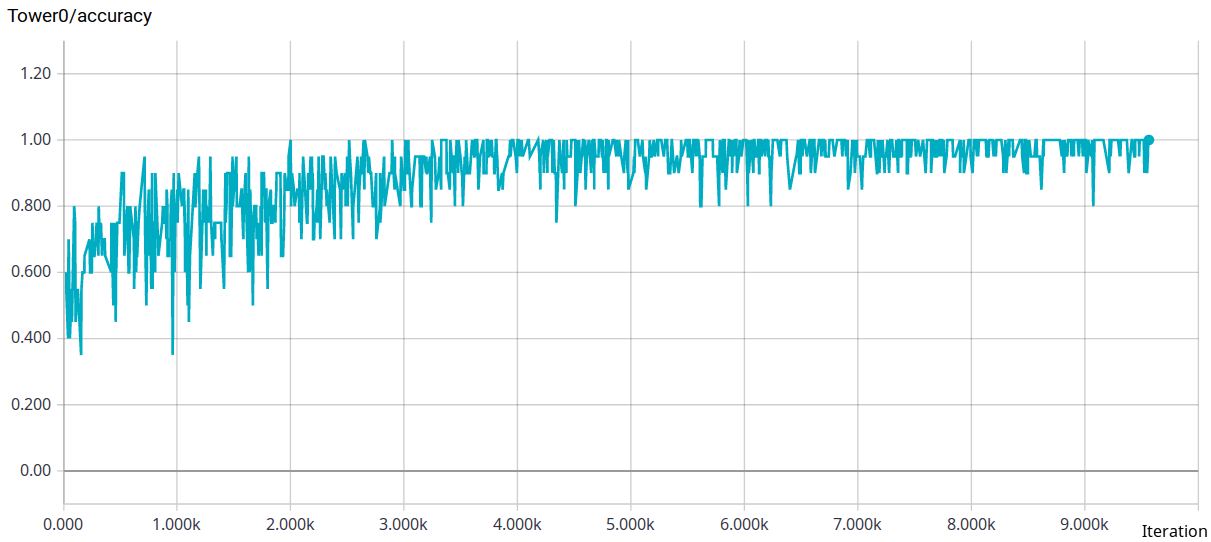
\includegraphics[width=\textwidth]{img_evaluation/pretrain2/tower0accuracy}
    \subcaption{Training accuracy of GPU0 (Tower0)}
    \end{subfigure}
    \begin{subfigure}[c]{\textwidth}
    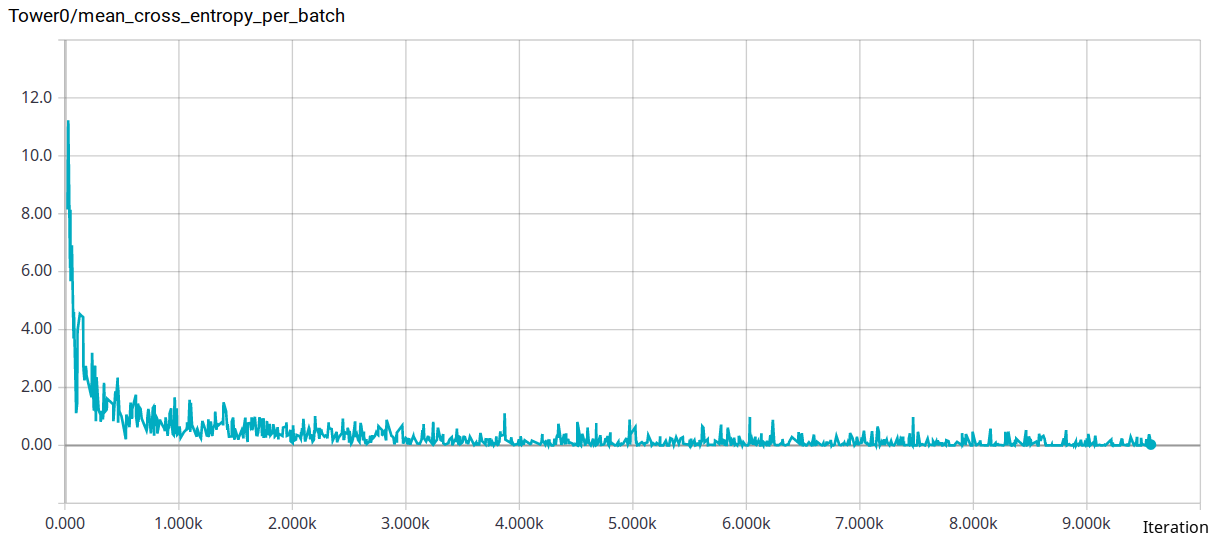
\includegraphics[width=\textwidth]{img_evaluation/pretrain2/tower0crossentropy}
    \subcaption{Training loss of GPU0 (Tower0)}
    \end{subfigure}
    \caption{Pre-training process by \textit{temporal order verification} using input sampling method 2.}
\label{fig:pretrain2}
\end{figure}

The pre-training process again converges fast in comparison to the pre-training times reported by \textcite{misra_shuffle_2016}.
In comparison to input sampling \textit{method 1}, training takes roughly three times longer.
This indicates, that sampling method 2 poses a more challenging learning task, since potential cuts need to be detected between every frame.
We therefore evaluate the quality of pre-training with \textit{method 2} by initializing a \textit{C3D} model from the pre-trained weights and train it on the Charades dataset.
Figure \ref{fig:pretrain2_initialized} shows training accuracy and loss per batch and training step on the Charades dataset for randomly initialized weights (blue) and training from pre-trained weights (yellow).

\begin{figure}[H]
    \begin{subfigure}[c]{\textwidth}
    \centering
    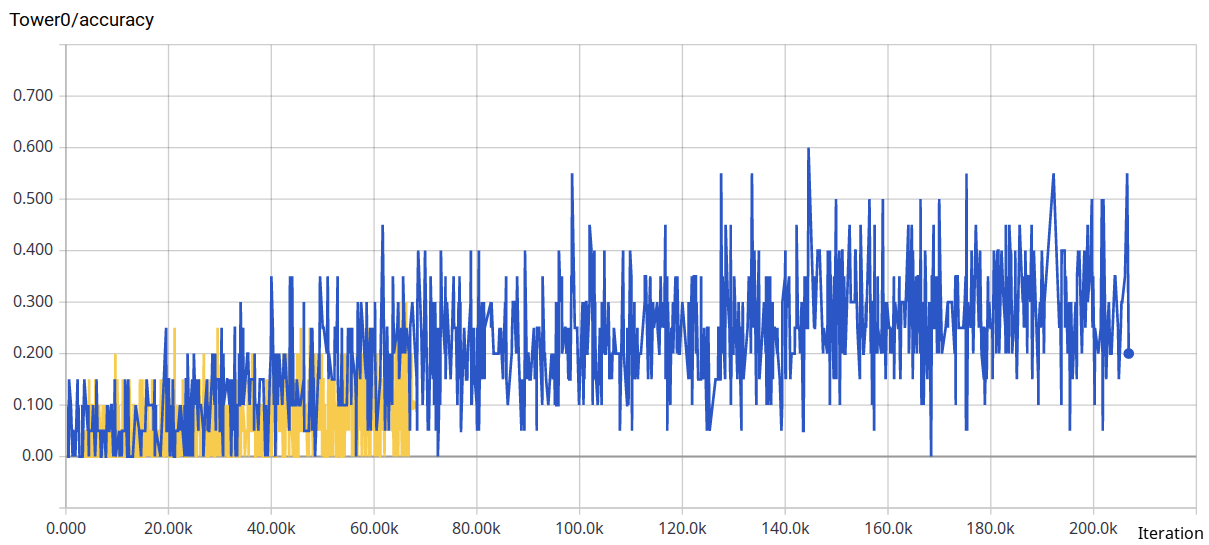
\includegraphics[width=\textwidth]{img_evaluation/pretrain2_initialized/tower0accuracy}
    \subcaption{Training accuracy of GPU0 (Tower0)}
    \end{subfigure}
    \begin{subfigure}[c]{\textwidth}
    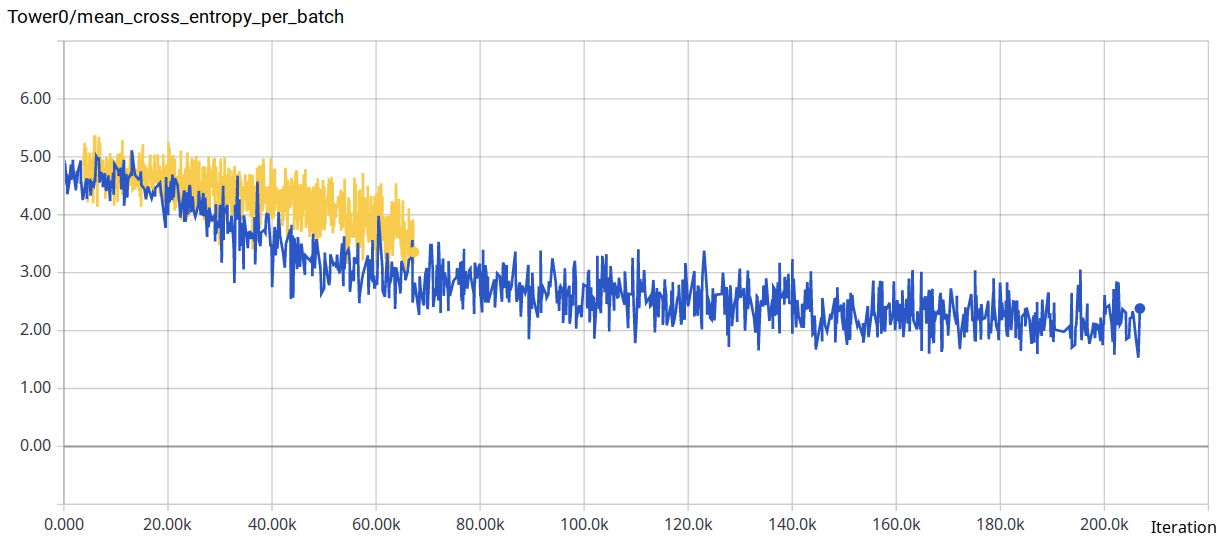
\includegraphics[width=\textwidth]{img_evaluation/pretrain2_initialized/tower0crossentropy}
    \subcaption{Training loss of GPU0 (Tower0)}
    \end{subfigure}
    \caption{Training a \textit{C3D} model on the Charades dataset from randomly initialized weights (\textit{blue}) and from pre-trained weights obtained through \textit{temporal order verification} (\textit{yellow}).}
    \label{fig:pretrain2_initialized}
\end{figure}

The progression of training accuracy and loss in figure \ref{fig:pretrain2_initialized} shows, that both models initially perform equally well. 
However, the pre-trained model performs significantly worse after iteration $15$k.
Specifically, the training loss of the pre-trained model is consistently higher than from the model without pre-training and the training accuracy is accordingly inferior.
This goes against the observation of pre-training in \cite{misra_shuffle_2016}, as the pre-trained model should require considerably less training steps to perform equally well or better during training and outperform the randomly initialized model during testing.
After a training time of roughly $2$ days, when the performance deficit was significantly noticeable, the training was stopped.
We therefore concluded pre-training with input sampling \textit{method 2} to be non beneficial for action recognition and focus on \textit{method 3}.
\bigskip

% continue reading here
\textbf{Method 3}\\
This sampling method is, compare to the previous two, most sophisticated and related to the original approach of \textcite{misra_shuffle_2016}.
As the \textit{C3D} model is replicated three times in a triplet siamese network, also the inputs are three times bigger.
This necessitates a decrease of the batchsize, in our case to $16$ input examples per training step, to not exceed the GPU memory.

The model was pre-trained for $83.13$k iterations, which corresponds to 2 days 20 hours 56 minutes and 2 seconds with a batchsize of $16$ examples.
The training accuracy quickly adjusts to a mean training accuracy of around $75\%$, yet does not change noticeably over the pre-training process.

\begin{figure}[H]
    \begin{subfigure}[c]{\textwidth}
    \centering
    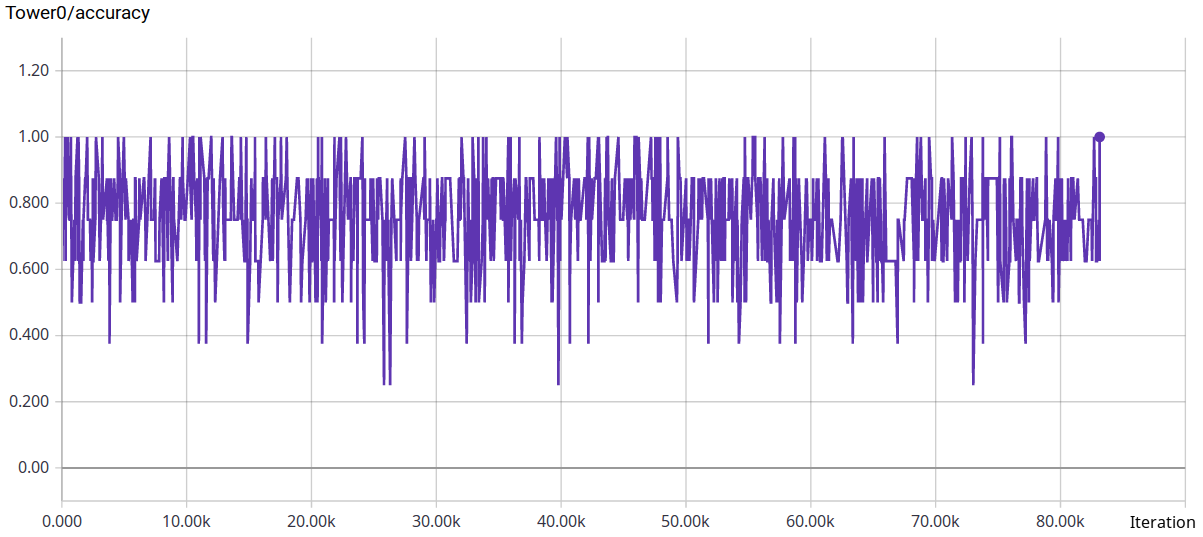
\includegraphics[width=\textwidth]{img_evaluation/pretrain3/tower0accuracy}
    \subcaption{Training accuracy of GPU0 (Tower0)}
    \end{subfigure}
    \begin{subfigure}[c]{\textwidth}
    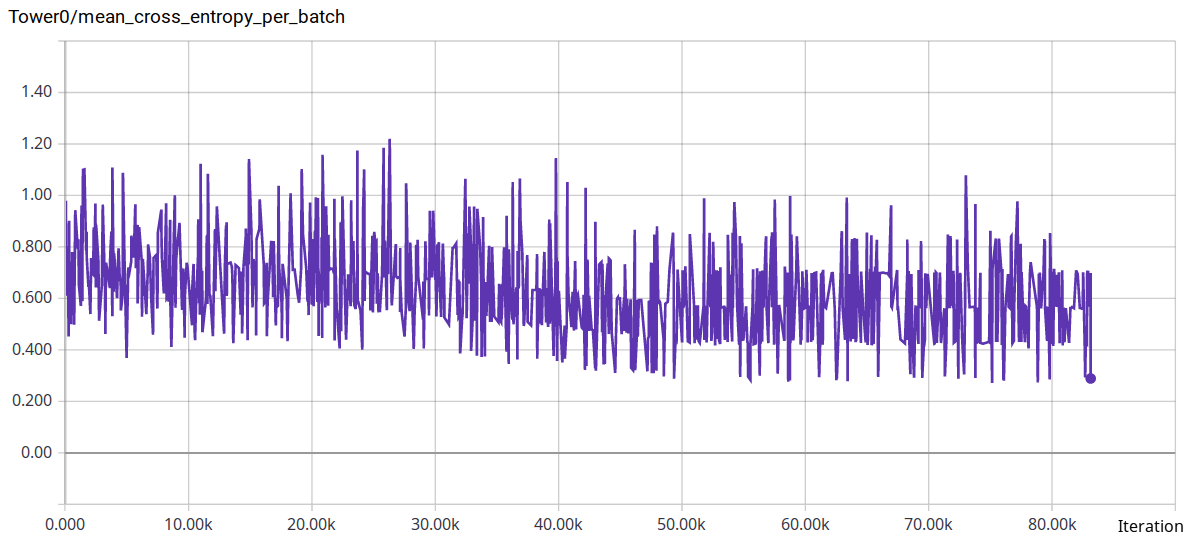
\includegraphics[width=\textwidth]{img_evaluation/pretrain3/tower0crossentropy}
    \subcaption{Training loss of GPU0 (Tower0)}
    \end{subfigure}
    \caption{Pre-training process by \textit{temporal order verification} using input sampling method 3.}
    \label{fig:pretrain3}
\end{figure}

The fact, that the training accuracy does not noticeably improve during the training, might raise the concern that no weight updates are taking place and the training process is inherently flawed.
However, the apparent decrease in training loss indicates weight updates, which have been confirmed by manual checking of parameters across multiple saved models.
\textcite{misra_shuffle_2016} report an accuracy of $72.1\%$ for \textit{temporal order verification}, which is comparable to our observation.
We therefore evaluate the last saved model from this pre-training run for supervised fine-tuning on UCF-101 and Charades.

\subsection{UCF-101 Classification with Pre-Training}
To evaluate the weights obtained by input sampling method 3, a \textit{C3D} model is initialized on the previously obtained weights and trained for $24,139$ iterations, which corresponds to $100$ epochs on UCF-101 at a batch-size of $40$ input clips per iteration ($20$ inputs per GPU).
The overall training process takes 17 hours and 6 seconds. 

Figure \ref{fig:pretrain3initializedUCF101} illustrates the training process for the pre-trained model (yellow) in comparison to the previously trained model from randomly initialized weights (cyan).

\begin{figure}[H]
    \begin{subfigure}[c]{\textwidth}
    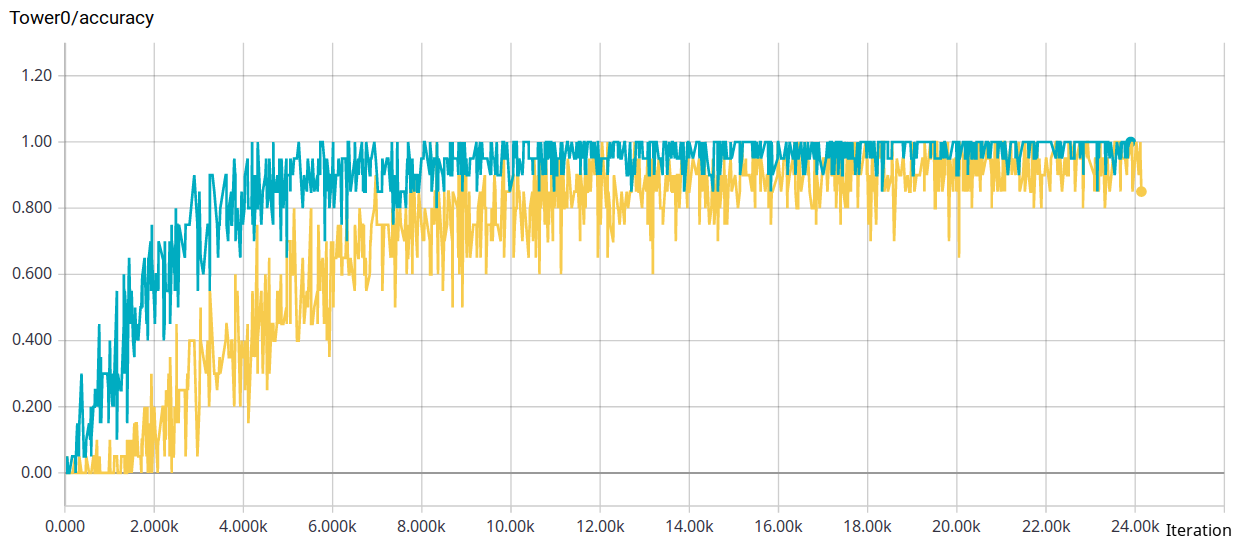
\includegraphics[width=\textwidth]{img_evaluation/pretrain3_initialized/tower0accuracy}
    \subcaption{Training accuracy of GPU0 (Tower0)}
    \end{subfigure}
    \begin{subfigure}[c]{\textwidth}
    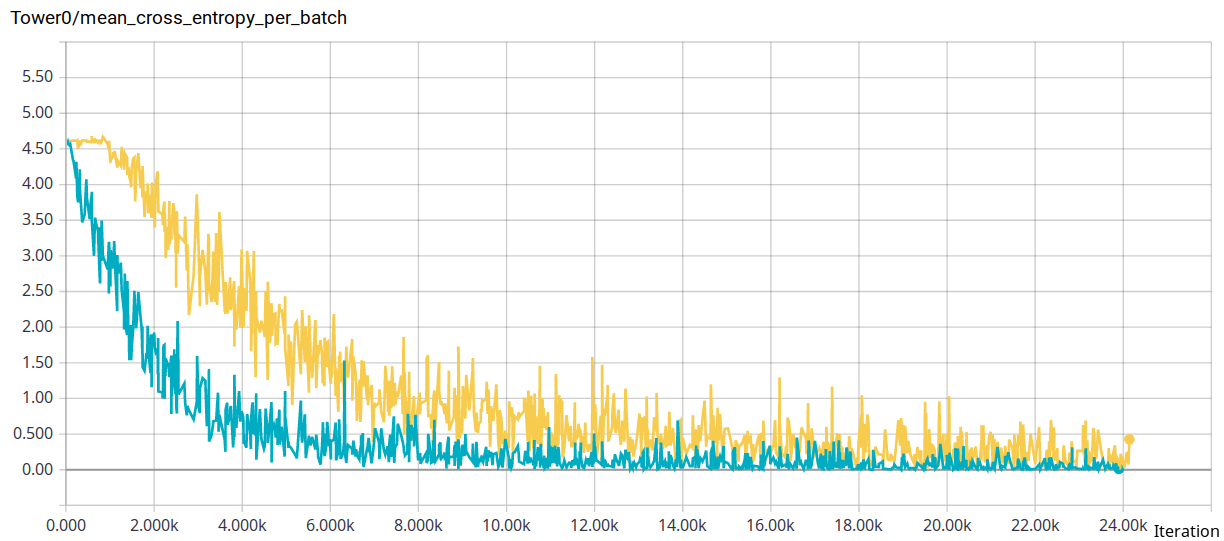
\includegraphics[width=\textwidth]{img_evaluation/pretrain3_initialized/tower0crossentropy}
    \subcaption{Training loss of GPU0 (Tower0)}
    \end{subfigure}
    \caption{Training process of a \textit{C3D} model from randomly initialized weights (cyan) in comparison to training a \textit{C3D} model from pre-trained weights obtained by pre-training method 3.}
    \label{fig:pretrain3initializedUCF101}
\end{figure}

The progression of training accuracy and loss curve indicates a slower training process compared to training the model without pre-training.
The curves obtained from pre-training converge close to the optima, yet not as strictly as before.
Since the model without pre-training overfit to the training data, this might indicate a regularization effect of pre-training the model.

\textbf{Result:}\\
We evaluate the pre-trained model on the test set of UCF-101.
Epoch ?? results in the best performing model, which yields an accuracy of ??.
This result is significantly worse than training the model from randomly initialized weights, which yields an accuracy of $44.57\%$.
The previously conjectured regularization effect is therefore not present and pre-training the model actually impairs the performance of the model.
The loss curve of the pre-trained model in figure \ref{fig:pretrain3initializedUCF101} (b) shows a plateau at the beginning of training.
This is due to the disadvantageous initialization and the optimizer adjusts the initial weights without any change in training loss.


\subsection{Charades Classification with Pre-Training}
The effect of the pre-trained weights obtained with method 3 is additionally evaluated on the Charades dataset.
A \textit{C3D} model is initialized on the previously obtained weights and trained for $31.15$k iterations, which corresponds to $24$ finished iterations.

Figure \ref{fig:pretrain3initializedcharades} illustrates the training process compared to training on the charades dataset from randomly initialized weights.
The initial plateau in the training loss is clearly identifiable.
After $1$ day $2$ hours and $56$ minutes the training process was stopped due to time constraints.
However the time-span is long enough to also confirm the negative effect of pre-trained weights on the Charades dataset.

\begin{figure}[H]
    \begin{subfigure}[c]{\textwidth}
    \centering
    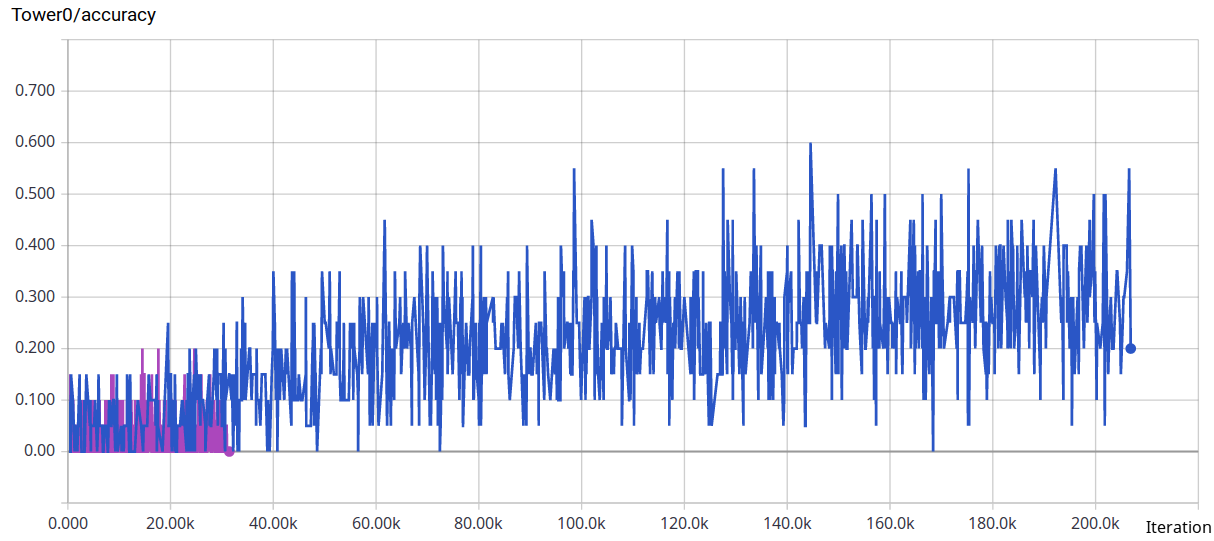
\includegraphics[width=\textwidth]{img_evaluation/pretrain3_initialized_charades/tower0accuracy}
    \subcaption{Training accuracy of GPU0 (Tower0)}
    \end{subfigure}
    \begin{subfigure}[c]{\textwidth}
    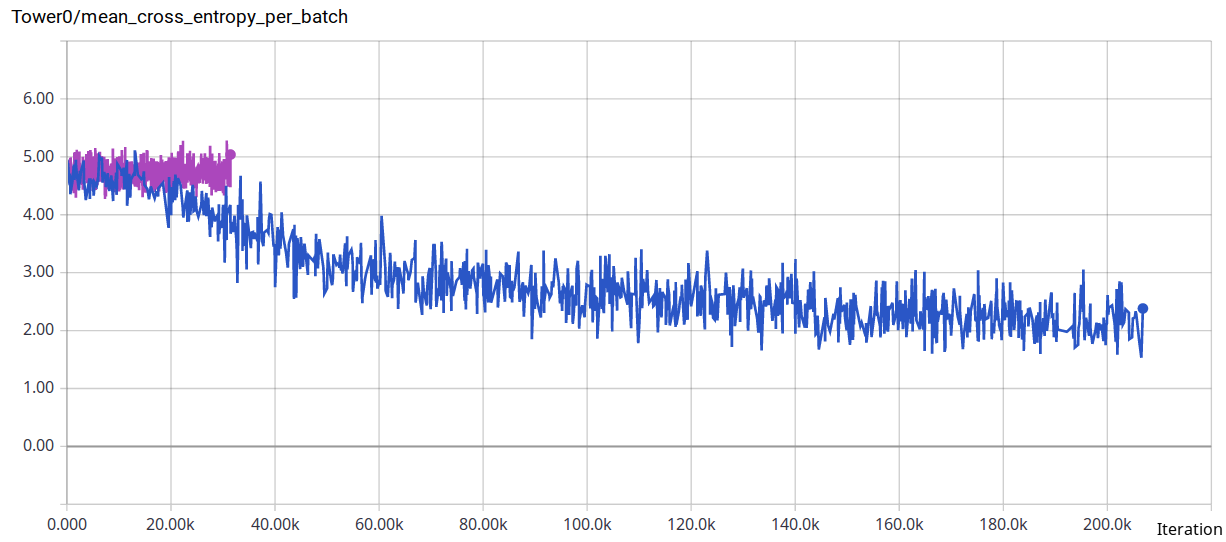
\includegraphics[width=\textwidth]{img_evaluation/pretrain3_initialized_charades/tower0crossentropy}
    \subcaption{Training loss of GPU0 (Tower0)}
    \end{subfigure}
    \label{fig:pretrain3initializedcharades}
    \caption{Training of a \textit{C3D} model on the Charades dataset from pre-trained weights (purple) compared to training from randomly initialized weights (blue).}
\end{figure}

\subsection{Discussion}
As these results disprove our initial hypothesis, that one of the above evaluated input sampling strategies can be used to beneficially transfer \textit{temporal order verification} to 3D CNNs, we investigate probable causes.
Upon manually investigating the Kinetics source videos, which were used to sample positive and negative examples for \textit{Temporal Order Verification}, we identified several of these to contain cutscenes.
Since the magnitude of contained motion is evaluated by splitting an input clip into three parts and comparing the similarity of between each chunk's mean frame, a pre-existing cutscene would identify the input as a high motion video clip.
This would then compromise the labelling during \textit{temporal order verification}, because an non permuted input clip with a cutscene is labelled as \textit{correct temporal order} although being de-facto temporally discontinuous.


\newpage
\section{Conclusion and Future Directions}
In this work we studied the quasi unsupervised pre-training method called \textit{temporal order verification} for improving the recognition of daily living actions from video data with a deep 3D convolutional neural network, i.e. the \textit{C3D} network model.
\textit{Temporal order verification} has shown promising results in learning movement-focused representations from still video frames with 2D CNNs. 
We therefore evaluated it as a means to incorporate motion sensitivity in 3D convolutional neural networks, which otherwise treat the temporal evolution of a video equally to the spatial dimension of video frames.
Two-stream CNNs address this issue by explicitly incorporating optical flow, which is computationally expensive to obtain.
Since pre-training a network with \textit{temporal order verification} does not require labelled data, it is especially suited to improve recognition tasks where large amounts of labelled data are sparse.
Specifically we focused on the Charades dataset, which features a unique amount of mundane daily-living action videos and therefore enables vision-based systems, which can can deployed in real-world applications such as assistive robotics.

In this work we devised an asynchronous input pipeline for multiple GPUs to make deep neural network training for action recognition from video data feasible on commercial hardware.
We trained the \textit{C3D} model for action recognition using this pipeline on multiple GPUs in a data parallel way, which yields competitive performance in recognizing daily-living actions.
We additionally studied three different input sampling methods to transfer the procedure of \textit{temporal order verification} from 2D CNNs into 3D CNN pre-training.
The first two methods focus on permuting single network inputs for a single \textit{C3D} model.
The third method adapts the replication of network models and processes three network inputs, which are individually kept unchanged but whose temporal order amongst each other is permuted.

By incorporating multiple GPUs in the training process and feeding input data through our input pipeline we were able process ?? times more input clips per second compared to training on a single GPU.
Our \textit{C3D} implementation yields an accuracy of ?? on the UCF-101 action recognition standard benchmark and a mean average precision of ?? for recognizing daily-living actions of the Charades dataset.
The longest training duration in the course of this work took $7$ days and $11$ hours on two GPUs, which would have been prolonged to ?? by training on a single GPU only.
We conclude that efforts to reduce training time are vital for action recognition research, since more training runs and evaluations can be performed in a given amount of time.

By pre-training the \textit{C3D} network with \textit{temporal order verification}, we were not able to improve the action recognition performance with any of the three evaluated input sampling methods.
The pre-trained weights turned out to significantly impair the network's performance.
This result underlines the impact of weight initializations on the ability of a network to effectively learn a classification task and fuels the future search for proper initialization methods to improve a network's performance.
We hypothesize, that the observed decrease in performance may be due to pre-existing cutscenes in the source videos, which were not introduced from permuting inputs and therefore compromise the generation of positive samples with \textit{correct temporal order}.
This could be addressed by first detecting pre-existing cut scenes in a source video and sampling \textit{temporal order verification} input clips only from continuous regions of the video.

In the course of this work we identified additional aspects to improve action recognition performance in the future.
A human detector could be incorporated to provide the learning system with more relevant training clips during training, instead of sampling input clips randomly from a training video.
As this does not heavily influence training on pre-processed datasets, which contain clips of a single human performing a single action, it would provide better training inputs for real-world training datasets.
We initially chose the \textit{C3D} model for this work, because it's deficits are potentially addressed by \textit{temporal order verification} and since it is a prominent example of a single stream 3D CNN, results can be compared to other publications in action recognition that picked up the model.
However, several recent advances such as strided convolutions to substitute the pooling layers for dimensionality reduction or skip-connections could be incorporated.
Most importantly a longer temporal extent, i.e. temporally longer inputs should be processed by the model as this was found to heavily influence action recognition performance.
To stay computationally feasible the final fully-connected layer would then need to be reduced in size.
